\section{Background}
\label{sec:background}

In this section background information is presented for the relevant topics to this thesis study. Process discovery approaches and then mismatch patterns in process models are presented. All topics in this chapter are limited to the scope of this thesis study with the aim of constructing a necessary background.

In process mining field, one of the most challenging tasks is to construct a process model based on the behavior in the event logs, namely process discovery. Many process discovery algorithms are proposed to address different challenges in process discovery and using different notations. However, in this study focus of the study is learning from the cross-organizational process mining rather than addressing all process discovery challenges. With this reasoning, Inductive Process Mining \cite{leemans2013discovering} is selected as appropriate since it is simple, highly applicable and configurable. In the literature, its derivatives which handles infrequent behaviors \cite{leemans2014discoveringinfrequent}; incomplete logs \cite{leemans2014discoveringincomplete}; and model optimization \cite{weidlich2012profiles} are also available. \textit{Inductive Miner Infrequent (IMi)} \cite{leemans2014discoveringinfrequent} extension is used in this study which is capable of filtering the infrequent behavior and results with lower fitness, higher precision and equal generalization.

In cross-organizational process mining environment, there is a need to align processes of different organizations and in this scope both the organizations and their processes are similar but have significant differences. In order to align these processes and organizations, there is a need for spotting differences between process models. In the study of Dijkman \cite{dijkman2007mismatch}, a collection of patterns to describe frequent mismatches between the similar process models are presented. Mismatch patterns are grouped into three as authorization, activity and control flow mismatch patterns. Authorization mismatch patterns are based on assignment of the same tasks to different roles in different processes and left outside the scope of this thesis. Activity mismatch patterns are based on representing the tasks of a process by a different collection of activities in a different process, or not representing at all. Within the scope of this study, the related activity mismatch patterns are defined in study \cite{dijkman2007mismatch} as follows:
\begin{description}
  \item[Skipped Activity] An activity exists in one process but no equivalent activity is found in the other process as illustrated in Figure~\ref{fig:skipped-activity}.
      \begin{figure}
      \centering
      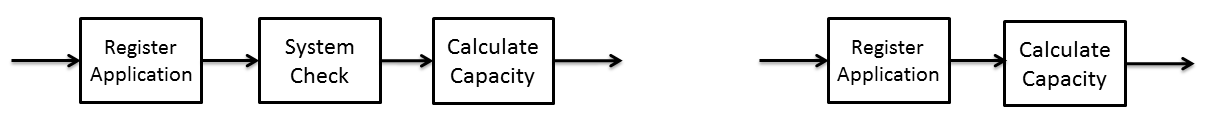
\includegraphics[width=\textwidth]{3_background/mismatch-patterns-skipped-activity}
      \caption{Example of Skipped Activity Pattern}
      \label{fig:skipped-activity}
      \end{figure}
  \item[Refined Activity] An activity exists in one process but, as an equivalent, a collection of activities are existing in the other process to achieve the same task. An illustration is provided in Figure~\ref{fig:refined-activity}. 
      \begin{figure}
      \centering
      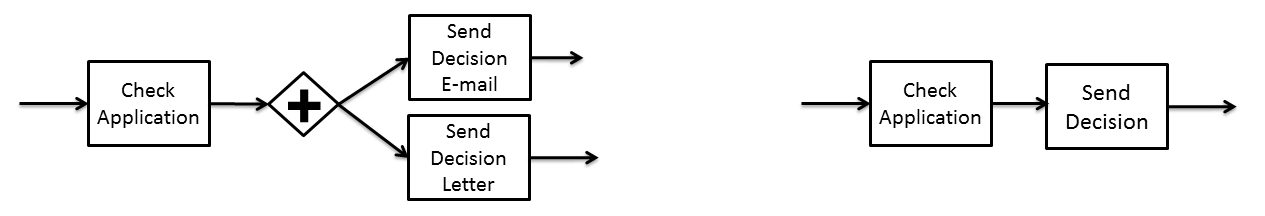
\includegraphics[width=\textwidth]{3_background/mismatch-patterns-refined-activity}
      \caption{Example of Refined Activity Pattern}
      \label{fig:refined-activity}
      \end{figure}
\end{description}
 
Control flow mismatch patterns are based on using different control-flow relations and dependencies for the same activities in different processes. Within the scope of this thesis study, the following related control flow mismatch patterns are defined as given in \cite{dijkman2007mismatch}:
\begin{description}
  \item[Activities at Different Moments in Processes] Set of activities are undertaken with different orders in different processes as shown in Figure~\ref{fig:different-moments}. 
      \begin{figure}
      \centering
      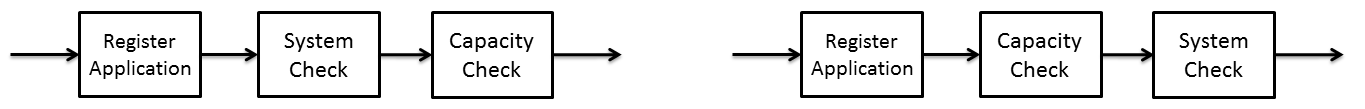
\includegraphics[width=\textwidth]{3_background/mismatch-patterns-different-moments}
      \caption{Example of Activities at Different Moments in Process Pattern}
      \label{fig:different-moments}
      \end{figure}
  \item[Different Conditions for Occurrence] Set of dependencies are same for two processes; however, occurrence condition is different. An example is provided in Figure~\ref{fig:different-conditions}.
      \begin{figure}
      \centering
      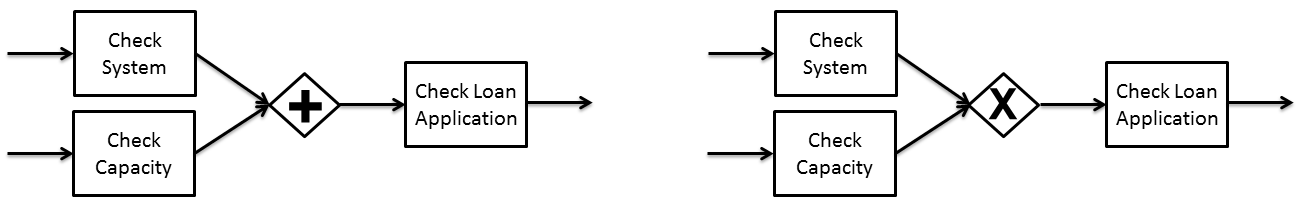
\includegraphics[width=\textwidth]{3_background/mismatch-patterns-different-conditions}
      \caption{Example of Different Conditions for Occurrence Pattern}
      \label{fig:different-conditions}
      \end{figure}
  \item[Different Dependencies] Dependency set of activities differ in different organizations. An example of this pattern is shown in Figure~\ref{fig:different-dependency}.
      \begin{figure}
      \centering
      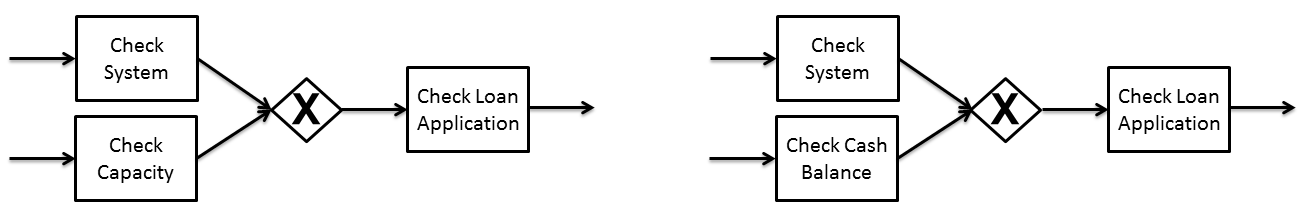
\includegraphics[width=\textwidth]{3_background/mismatch-patterns-different-dependency}
      \caption{Example of Different Dependencies Pattern}
      \label{fig:different-dependency}
      \end{figure}
  \item[Additional Dependencies] This pattern is a special case of different dependencies where one set of activities includes the other and results with additional dependencies as illustrated in Figure~\ref{fig:additional-dependency}.
      \begin{figure}
      \centering
      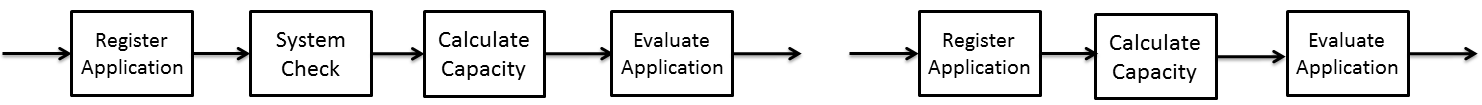
\includegraphics[width=\textwidth]{3_background/mismatch-patterns-additional-dependency}
      \caption{Example of Additional Dependencies Pattern}
      \label{fig:additional-dependency}
      \end{figure}
\end{description}

As mentioned in the study \cite{dijkman2007mismatch}, their approach does not create a comprehensive list to resolve all mismatches but the most common ones spotted during case studies. In addition, from their definitions and examples it can be easily seen that these patterns are not orthogonal. Moreover, there are no algorithms provided to spot these mismatches in \cite{dijkman2007mismatch} or consequent studies, and thus implementation of spotting mismatch patterns are kept within the scope of this thesis study.